%!TEX root = ../Work-stealing Queues.tex
\section{Background}
\label{sec:background}

This section presents the concepts underlying the queue implementations and the subsequent analysis. In particular, different approaches to creating concurrent application are discussed.

\subsection{Common Concurrency Problems}
Many errors can arise which are directly caused by the presence of concurrent computations. One of the most important problems related to work-stealing queues is the \emph{ABA problem}. This problem can occur in the context of a \emph{compare-and-swap} operation, where the update is performed if the value of the given register is as expected. However, this provides no guarantees that the value has not changed since we last observed it, and then been changed back by another thread. Thus, the ABA problem gets its name from the notion that the register was \emph{A} when we observed it, but then changed to \emph{B} and back to \emph{A} before our next observation. In some situations we need to prevent this from happening, which may require specific measures to be taken.

Another common problem is \emph{check-then-act}. This problem can arise if a thread is supposed to perform some action as a consequence of the successful result of a check. If the thread first performs the check successfully, but is then suspended by the scheduler, then the result of the check might no longer be valid when the thread is later resumed, since other threads could have made changes to the shared state in the meantime. In such case, the invariants of the system could be violated if the planned action is performed by the resumed thread.

\subsection{Approaches to Concurrency}
The complexity of building concurrent applications arises mostly from the inherent need to manage concurrent access to shared state, in particular shared \emph{mutable} state. With shared mutable state, any thread may write to any memory location at any time (in principle), which makes maintaining the invariants of the system a major concern. Keeping shared state immutable eliminates many such problems, as no threads will ever read different data from the same memory location at different moments in time. While it is arguably easier to reason about concurrent applications with immutable shared state, having mutable state can be desirable for several reasons, the most compelling of which is (possible) increased performance. In the following, we will discuss different approaches to handling concurrent access to shared mutable state.

% locks
\subsubsection{Lock-based Synchronization}
Locking is a widely used mechanism for handling access to shared mutable state, especially in the realm of imperative programming. Locks can be used to grant exclusive access to one or more shared resources by associating that resource with a lock (assuming a locking scheme with \emph{mutual exclusion locks}, where a given lock can only be held by one thread at a given point in time). The problem of synchronization is solved by a guarantee that no other threads will be accessing the shared resource as long as the lock is being held. Since any access to the resource must be exclusive, a lock must be obtained both when reading from and writing to it. 

While the exclusive locking mechanism preserves the integrity of the shared state, this exclusivity is also one of the greatest disadvantages of locking. Whenever a thread tries to obtain a lock held by another thread, the call blocks and the thread is suspended and must wait (potentially forever) for the current lock owner to finish its work. During this time, the waiting thread cannot do anything else. For locks under high contention, the performance degradation caused by the overhead of suspending and resuming threads might be very high, especially if the lock is only required for reading. For these situations, the use of non-blocking synchronization can be preferable.


% blocking vs. non-blocking queues
\subsubsection{Non-blocking Synchronization}
Instead of taking the pessimistic approach of making sure that exclusive access is obtained before performing any operations on a shared resource, non-blocking synchronization is more optimistic in nature\,\citep{Goetz2006}. Being \emph{non-blocking} means that if a thread fails or is suspended, it cannot cause another thread to fail or be suspended, because threads accessing a shared resource never have to wait for another thread (contrary to the lock-based scheme, where a thread may have to wait for the release of a lock)\,\citep{Goetz2006}. A non-blocking algorithm can be said to be \emph{lock-free}, which means that at any point of execution, some thread is making progress (and thus the term has nothing to do with lock-based synchronization).

In the non-blocking scheme, the integrity of a shared resource is ensured by only allowing updates to happen atomically from a consistent state, where all the invariants of the system hold. If some invariant does not hold, e.g. when a shared variable has another value than expected because it has been updated by another thread, a recovery mechanism is triggered instead. To perform atomic non-blocking updates, specific processor instructions (e.g. compare-and-swap) must be used to avoid common concurrency problems such as \emph{check-then-act}. 

Non-blocking synchronization provides a more fine-grained approach to synchronization, where the cost of suspending and resuming threads is replaced by the need for a recovery mechanism when faced with failed updates (retrying is a perfectly valid recovery mechanism). However, a non-blocking algorithm can be more complicated to design than a similar lock-based one\,\citep{Goetz2006}, so using non-blocking synchronization might not always be desirable.

% Here, specific processor instructions (e.g. \emph{compare-and-swap}) are used to perform atomic compound operations on shared resources, but in contrast 

% Non-blocking synchronization utilizes hardware support to ensure the integrity of shared state. Instead of using locks to perform atomic compound operations, specific processor instructions, such as \emph{compare-and-swap}, are used to make sure that updates to shared resources only happen from a consistent state. As opposed to exclusive locking, non-blocking operat

% As opposed to the pessimistic approach of locking, where all locks must be obtained before 
% lock-free vs. wait-free ?

\subsection{A Simple Solution}
The simplest solution to the problem of concurrently processing \emph{n} suspended computations (denoted ``work units'' or simply ``work''), is to have \emph{m} worker threads processing these in parallel from a central queue. To avoid two threads handling the same work unit, a lock is placed on this central queue, which must be held in order for a thread to take more work. Whenever two or more threads finish their current work simultaneously, they will all try to obtain the lock from the queue. However, only one of them will succeed, and the others will be suspended while waiting for the lock. In these situations, many threads will be idle at any given time when contention for the lock gets high. Consequently, this design leads to a situation where the central work queue becomes a bottleneck, and computational resources are wasted while threads are idle. Although not very efficient, a simple design such as this can serve as a good baseline for comparison with other approaches.


\subsection{Work-stealing Queues} % What is a work-stealing queue?
A work-stealing queue is a queue implementation that facilitates working with work-stealing scheduling algorithms\,\citep{Arora:1998:TSM:277651.277678}. In a work-stealing scheduling algorithm, each thread is assigned a work-stealing queue, the elements of which are work units. This queue has the standard \texttt{push} and \texttt{take} operations for adding and removing elements from it, respectively, and only the thread owning the queue has access to these operations. Additionally, the queue exposes a \texttt{steal} operation, through which other threads may ``steal work''. An example of such a scenario is shown in Figure~\ref{fig:workstealing_scenario}.

Work-stealing algorithms are especially well-suited for solving problems where one unit of work may generate more work (examples of which can be found in Section \ref{sec:benchmarks}). The idea is that whenever the work unit processed by a given thread generates more work, this work is stored in the thread's local queue. When the thread finishes its current work, it first examines its own queue, and continues to process any work it might find. If no work is found locally, the thread begins to examine the queues of other threads, in effect ``stealing'' the work generated by these. This design leads to efficient utilization of computation resources, since a thread is never idle: it is either working or looking for more work.

\begin{figure}
\begin{center}
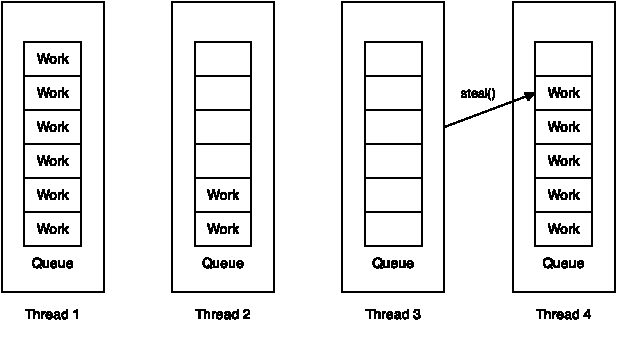
\includegraphics[scale=1]{resources/WSQ.pdf}
\end{center}
\caption{An example situation from a work-stealing algorithm with four working threads. Each thread has its own queue. Thread 3 has completed all of its own work, and is therefore in the process of stealing work from thread 4.}
\label{fig:workstealing_scenario}
\end{figure}

\subsection{Software Transactional Memory}
Software Transactional Memory (STM) is an attempt to address the difficulty of designing concurrent algorithms and data structures, by enabling the user to specify concurrent operations as transactions. Following the formulation of transactional memory presented by Herlihy and Moss\,\citep{HerlihyMossTM}, Shavit and Touitou proposed the first model for software-only transactional memory\,\citep{ShavitSTM}. Using STM, shared memory can be accessed and updated by means of transactions, where a transaction is understood as an application of a finite sequence of primitive operations to that shared memory. Furthermore, the transactions must have the properties of \emph{atomicity} (transactions appear to happen sequentially) and \emph{serializability} (the sequential order of transactions is consistent with their real-time order)\,\cite{ShavitSTM}.

Ideally, designing concurrent algorithm with STM should shift much of the burden of worrying about concurrency from the user to the runtime system, without incurring any performance trade-offs. A study done by Dice and Shavit\,\citep{Dice06whatreally} shows that algorithms implemented using STM scale better than equivalent hand-crafted algorithms, both lock-based and non-blocking. However, opponents of STM claim that it causes a higher sequential overhead than more traditional shared-memory approaches\,\citep{Cascaval08}, since transactions expand to many more load and store instructions, leading to performance losses.

In an improvement to their earlier algorithm, Dice, Shalev, and Shavit\,\citep{DiceTLII} present the \emph{Transactional Locking II} algorithm, which supposedly is ``an order of magnitude faster than sequential code made concurrent using a single lock.'' This is achieved using a global version-clock, which allows for fast read-only transactions. Although these findings seem promising, the debate concerning the performance of concurrent algorithms implemented using STM has yet to reach consensus.
